% !TeX spellcheck = ru_RU
%pdflatex, utf8
\documentclass[unicode, 10pt, a5paper, oneside]{article}

% Установка полей страницы
%\usepackage{anysize}
%\marginsize{0.3cm}{0.3cm}{0.3cm}{0.3cm}
\usepackage[a5paper, margin=0.3cm, bindingoffset=0cm]{geometry}

% Поддержка русского языка
\usepackage[T2A]{fontenc}		% Корректная кодировка шрифта при использовании cm-super
\usepackage[utf8]{inputenc}		% Кодировка ввода
\usepackage[russian]{babel}		% Словарь расстановки переносов
%\usepackage{cmap}				% Перекодировка символов в pdf при использовании обычного cm

% Всякие математические фишки
\usepackage{amsmath}
\usepackage{amsfonts}
\usepackage{amssymb}

% Изменение цвета, работа с графикой
\usepackage{color}
\usepackage[pdftex]{graphicx}
\graphicspath{{images/}}

% Команда для вставки ссылок \url{URL}
\usepackage[hyphens]{url}
\urlstyle{rm}					% Стиль шрифта ссылок: с засечками

% Кликабельные ссылки внутри документа
\usepackage[unicode]{hyperref}

% Включает отступ у первого абзаца в разделе
\usepackage{indentfirst}

% Настрйока стиля списков
\usepackage{enumitem}
\setlist{noitemsep, leftmargin=*, labelindent=\parindent, topsep=0pt, parsep=0pt, partopsep=0pt}

\setlist[itemize,1]{label=$\diamond$}
\setlist[itemize,2]{label=\textendash}
\setlist[itemize,3]{label=$\star$}

\renewcommand{\alph}[1]{\asbuk{#1}} % Костыль для кирилической нумерации вместо латинской
\setlist[enumerate,1]{label=\arabic*)}
\setlist[enumerate,2]{label=\alph*)}
\setlist[enumerate,3]{label=(\arabic*)}


\usepackage{textcomp}			% Команды для вставки разных символов (градусы, проценты, итд)
\usepackage{float}				% Размещение плавающих объектов там где они созданы (X)
\usepackage{wrapfig}			% Обтекаемые текстом рисунки

% Подписи у флоатов
\setlength{\intextsep}{0pt} % Отстут вокруг плавающих окружений
\usepackage{caption}
\captionsetup{parskip=0pt}
\captionsetup[figure]{labelsep=period,justification=centering,singlelinecheck=false,textfont=small,labelfont=small,aboveskip=2pt,belowskip=0pt}

% Изменение формата заголовков разделов
\usepackage{titlesec}
\titleformat{\section}{\newpage\small\bfseries}{\thesection. }{0pt}{}{}
\titlespacing*{\section}{0pt}{0pt}{0pt}

\titleformat{\subsection}{\small\bfseries}{\thesubsection. }{0pt}{}{}
\titlespacing*{\subsection}{0pt}{0pt}{0pt}

\usepackage{array}				% Позволяет объявить свои типы колонок
\usepackage{calc}				% Математика, исп-ся для расчёта ширины колонки
\usepackage{longtable}			% Длинные таблицы

% Минимальный отступ в таблицах
\setlength{\tabcolsep}{1.5mm}

% Новые типы колонок. Ширина задётся как доля от linewidth
\newcolumntype{L}[1]{p{#1\linewidth-2\tabcolsep-2\arrayrulewidth}}
\newcolumntype{C}[1]{>{\centering}p{#1\linewidth-2\tabcolsep-2\arrayrulewidth}}
\newcolumntype{R}[1]{>{\raggedleft}p{#1\linewidth-2\tabcolsep-2\arrayrulewidth}}
\newcolumntype{U}[2]{p{#1\linewidth-(#2)}}

% Стараться не оставлять одиноких строк в начале и конце абзаца
\clubpenalty=1000
\widowpenalty=1000

% Расстановка отступов и переносов
\emergencystretch=2.5em			% Максимальный промежуток между словами
\tolerance=2000
\frenchspacing


\begin{document}

\setcounter{section}{20}

% Вопрос 21 ---------------------------------------------------------------------------------------------------------------
\section{Дискретные цифровые САР: математическое описание, Z передаточные функции.}

Дискретными принято называть такие системы, в которых некоторые сигналы, передаваемые по каналам связи замкнутой системы, существуют только в отдельный момент времени или значение этих сигналов изменяется скачкообразно, ступенчато. Поэтому существует несколько типов дискретных систем, например, в которых производится квантование по уровню или по времени.

В цифровых системах управления квантование производится одновременно и по уровню и по времени. Значение сигнала существует в цифровой форме, соответствующей числу уровней в дискретные моменты времени.

\begin{center}
\texttt{Тут можно нарисовать квантование произвольной функции по уровню и по времени сначала отдельно, потом вместе.}
\end{center}

Обычно дискретная система управления строится по следующему принципу:

\begin{figure}[H]
\centering
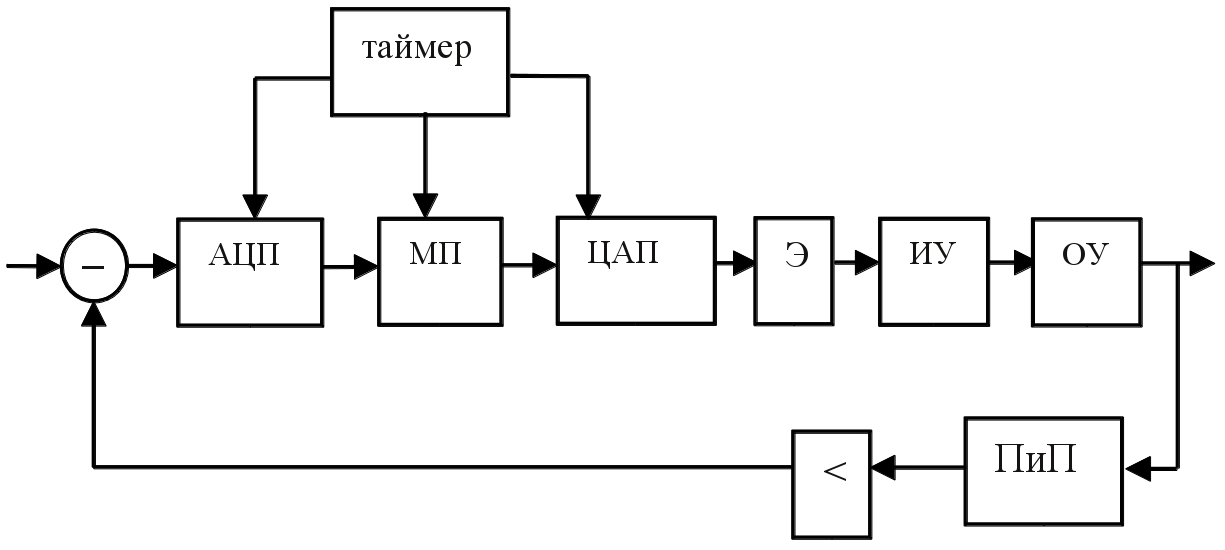
\includegraphics[width=0.7\linewidth]{21_dicret_struct.png}
\caption{Структура дискретной САУ: АЦП --- аналого-цифровой преобразователь, МП --- микропроцессор, ЦАП --- цифро-аналоговый преобразователь, Э --- экстраполятор, ИУ --- исполнительное устройство, ОУ --- объект управления, ПИП --- первичный измерительный преобразователь.}
\label{fig:21_dicret_struct}
\end{figure}

Дискретизация по времени приводит к тому, что система как замкнутая работает только в дискретные моменты времени. Поэтому упрощенная структура цифровых систем управления после линеаризации и структурных преобразований может быть представлена в виде совокупности линейной части и ключевого элемента.

Такое упрощение возможно благодаря высокому быстродействию современных вычислительных средств, то есть такая структура не учитывает запаздывания, создаваемого вычислительной процедурой.

\begin{figure}[H]
\centering
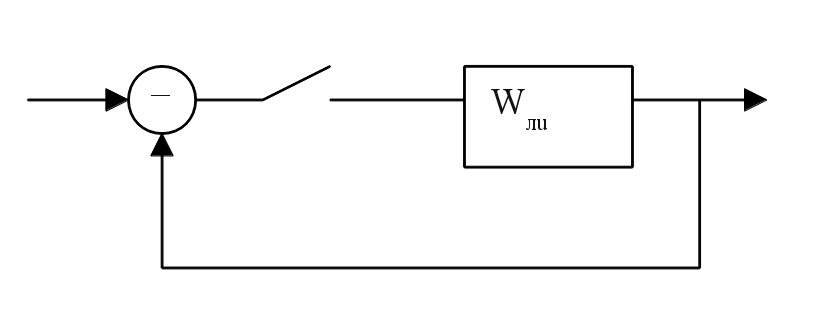
\includegraphics[width=0.5\linewidth]{21_dicret_struct_small.png}
\caption{Упрощённая структура дискретной САУ}
\label{fig:21_dicret_struct_small}
\end{figure}

\subsection*{Математическое описание дискретных систем}

Непрерывному сигналу $ x(t) $ в дискретных системах ставится в соответствие сигнал, соответствующий дискретному моменту времени:

\begin{equation}
x(t) \rightarrow x(k\tau_r) \text{, где}
\end{equation}
\par $ k = 0, 1, 2, \ldots $;\nopagebreak
\par $ \tau_r $ --- период дискретизации.

Математическое представление дискретных систем сводится к представлению ДУ с помощью упрощенных процедур \textit{вычисления конечных разностей}.

Если в непрерывной системе вычисление первой производной представляется с помощью ДУ, то в дискретной системе $ \left( \dfrac{dx}{dt} \rightarrow \dfrac{\Delta^1x}{\tau_r} \right)  $  --- первая разность к периоду дискретизации:
\begin{equation}
\Delta^1x = x((k + 1)\tau_r) - x(k\tau_r).
\end{equation}

Для вычисления второй производной можно использовать равенство:
\begin{equation}
\left( \dfrac{d^2x}{dt^2} = \dfrac{\Delta^2x}{\tau^2_r} \right) \text{, где}
\end{equation}
\par $ \Delta^2x = \Delta^1((k + 1)\tau_r) - \Delta^1(k\tau_r) $;\nopagebreak
\par $ \Delta^2 = x((k + 1)\tau_r) - x((k + 1)\tau_r) - x((k + 1)\tau_r) + x(k\tau_r) $.

Используя методы численного интегрирования с использованием разностных процедур можно получить следующее выражение, характеризующее дискретную САР:
\begin{equation}
y(k) = \sum_{i=0}^{m} x(k-m-i) - \sum_{j=0}^{n} y(k-n+i).
\end{equation}

Числа $y(k-n+i)$ и $x(k-m+j)$ характеризуют предыдущие значения выхода и входа ЦВМ, запоминаемые в памяти. Это уравнение называют \textit{рекурсивным или разностным}.

Реакция дискретной системы на дискретный сигнал так же может определяться с использованием принципа свертки функции:
\begin{equation}
y(k) = \sum_{k=0}^{n} x(k) w(k-n)\text{, где}
\end{equation}
\par $ w(k) $ --- весовая характеристика.

Это выражение --- аналог интеграла свёртки.

\subsection*{Z передаточные функции дискретных и цифровых САУ}

Z-преобразование получается путем замены переменных $ Z=e^{s\tau} $ в дискретных преобразованиях Лапласа, связывающих функцию $ F(s) $ комплексного переменного (изображение) с функцией $ f(x) $ вещественного переменного (оригинал). Z-изображение дискретных сигналов дает возможность найти соотношение между z-изображением входных и выходных дискретных сигналов.

Z-преобразование содержит информацию о соответствующей непрерывной  функции времени только в дискретные моменты, поэтому оно определяет не непрерывную функцию, а ряд ее последовательных дискретных значений:
\begin{equation}
X(z) = Z[x^*\tau] = \sum_{k=0}^{\infty} x(k\tau) Z^{-k}.
\end{equation}

Обратное Z-преобразование определяется формулой:
\begin{equation}
X^*(t) = Z^{-1} [X(z)] = \dfrac{1}{2\pi j} \oint\limits_r x(z) z^{k -1} dz
\end{equation}

Сигнал на выходе дискретных систем:
\begin{equation}
y(k) = \sum_{m=-\infty}^{\infty} w(k - m)g(m)\text{, где}
\end{equation}
\par $ w(k) $ --- весовая характеристика.

Передаточные свойства дискретной САР можно характеризовать с помощью \textit{дискретной передаточной функции}:
\begin{equation}
W(z) = \dfrac{Y(z)}{G(z)}\text{, где}
\end{equation}
\par $ Y(z) $ --- z-отображение выходного сигнала;\nopagebreak
\par $ G(z) $ --- z-отображение входного сигнала.

Для непрерывной части дискретной системы Z-передаточная функция определяется на основе соотношения:
\begin{equation}
W(z) = \sum_{k=0}^{\infty} w(k\tau) z^{-k} \text{, где}
\end{equation}
\par $ w(k\tau) = [w(t)]_{t=k\tau} $;\nopagebreak
\par $ k = 1, 2, 3, \ldots $;
\par $ w(t) = L^{-1} [w(s)] $.


% Вопрос 22 ---------------------------------------------------------------------------------------------------------------
\section{Анализ дискретных САР.}

Если в Z --- передаточной функции, дискретной САР с ЭВМ в контуре управления произвести замену:
\begin{equation}
W(z) = W_\text{в}(z) z[W_\text{в} W_\text{о} W_\text{ос}].
\end{equation}

Полагая, что передаточная функция обратной связи равна 1, что всегда можно обеспечить методом структурных преобразований, передаточную функцию контура можно представить в виде:
\begin{equation}
\Phi(Z) = \dfrac{W(z)}{1 + W(z)}.
\end{equation}

Таким образом, характеристическое уравнение одноконтурной дискретной системы с единичными обратными связями будет выглядеть:
\begin{equation}
1 + W(z) = 0.
\end{equation}

Устойчивость дискретных систем будет определяться корнями этого характеристического уравнения.

Для устойчивости \textit{непрерывных} систем необходимо чтобы корни располагались слева от мнимой оси. Для оценки устойчивости \textit{дискретных} систем производится переход из комплексной плоскости $ s $ в комплексную плоскость $ z $ с заменой  $ z = e^{\tau s} $. В этом случае мнимая ось $ s = j\omega $ комплексной плоскости $ s $ преобразуется в окружность с единичным радиусом, с центром в начале координат на комплексной плоскости $ z $.

На комплексной плоскости $ z $ уравнение мнимой оси: $ z = e^{i\tau\omega} = \cos\omega t + j\sin\omega t $.

\begin{figure}[H]
\centering
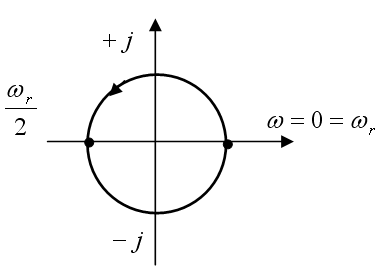
\includegraphics[width=0.4\linewidth]{22_circ.png}
$ \omega_r = \dfrac{2\pi}{\tau_r} $
\caption{Единичная окружность соответствующая $ s = j\omega $}
\end{figure}

Комплексные корни $ s_i = \alpha_i + j\beta_i $ соответствуют $ z_i = e^{\alpha_i\tau_r} + e^{j\beta_i\tau_r} $. Вещественная часть корня $ \operatorname{Re} (z_i) = e^{\alpha_i\tau_r} < 1 $, следовательно левая полуплоскость $ s $ отображается во внутреннюю часть единичной окружности.

Таким образом, дискретная система устойчива, если все корни характеристического уравнения располагаются внутри единичной окружности.


% Вопрос 23 ---------------------------------------------------------------------------------------------------------------
\section{Логарифмические частотные характеристики САР.}

В практике автоматики широкое применение находят частотные характеристики в логарифмических масштабах. Применение логарифмического масштаба позволяет наглядно изображать характеристики в большом диапазоне частот, представлять характеристики отрезками ломанных линии и определять характеристики сложных систем простым суммированием характеристик, входящих в эти системы элементов.

Частота в логарифмическом масштабе измеряется в декадах. \textit{Декада} --- диапазон частот между $ \omega $  и  $ 10\omega $:  $ \lg(\omega_\text{верх}/\omega_\text{нижн}) = 1 $.

\textit{Октава} --- диапазон частот между  $ \omega $ и  $ 2\omega $: $ \lg(\omega_\text{верх}/\omega_\text{нижн}) = \lg 2 $.

Широко используются логарифмические амплитудная (ЛАЧХ) и фазовая (ЛФЧХ) частотные характеристики (см. рис.). Они получаются путем логарифмирования передаточной функции:
\begin{equation}
\lg[W(j\omega)] = \lg[A(\omega)\exp(j\varphi(\omega))] = \lg[A(\omega)] + \lg[\exp(j\varphi(\omega))] = L(\omega) + \varphi(\omega).
\end{equation}

\textit{ЛАЧХ} получают из первого слагаемого, которое умножается на 20, то есть $ L(\omega) = 20 \lg A(\omega) $. Величина $ L(\omega) $ откладывается по оси ординат в децибелах. По оси абсцисс откладывается частота $ \omega $ в логарифмическом масштабе.

\textit{ЛФЧХ}, получаемая из второго слагаемого, отличается от ФЧХ только масштабом по оси $ \omega $. Величина $ \varphi(\omega) $ откладывается по оси ординат в градусах или радианах.

\textbf{Пример:} рассмотрим ЛАЧХ и ЛФЧХ апериодического звена первого порядка.
\begin{equation}
w(s) = k \dfrac{1}{Ts + 1}.
\end{equation}

Наклон ЛАЧХ -20 дБ/дек. Фаза стремится к $ -\pi/2 $.

\begin{figure}[H]
\centering
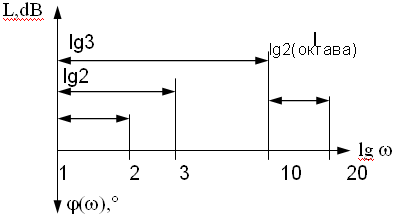
\includegraphics[width=0.7\linewidth]{23_lchars.png}
\caption{Логарифмические характеристики апериодического звена первого порядка}
\end{figure}

Частотные характеристики являются исчерпывающими характеристиками системы, по которым можно восстановить ее передаточную функцию и определить параметры.

Графический метод широко применяется для анализа параметров САР.
\begin{enumerate}
\item При $ 0 < \omega < \omega_c $, $ A(\omega) > A(0) $ и диапазон частот от 0 до $ \omega_c $ называется  полосой пропускания, где $ \omega_c $ --- частота среза по уровню $ A(j\omega) = 0 $ или $ A(j\omega) = 0,707 A(0) $;
\item При $ \omega = \omega_m  $, $ A(\omega) $ принимает максимальное значение и $ \omega_m $ называемое \textit{резонансной частотой}.
\end{enumerate}


% Вопрос 24 ---------------------------------------------------------------------------------------------------------------
\section{Переходные функции и переходные характеристики САР. Реакция САР на произвольный входной сигнал.}

Переходной функцией САР (или звена) называют функцию h(t), описывающую реакцию системы на единичное ступенчатое воздействие  при нулевых начальных условиях. График этой функции называют переходной характеристикой.

Импульсной переходной или весовой функцией (функцией веса) называют функцию w(t), описывающую реакцию САР (звена) на единичное импульсное воздействие при нулевых начальных условиях. График этой функции называют импульсной переходной характеристикой.

При единичном ступенчатом воздействии входная величина мгновенно возрастает от 0 до 1 и далее остается неизменной, т.е. 

$$ 1(t)=\left\{
	\begin{array}{rcl}
	 0,t<0\\
	 1,t\geq 0\\
	\end{array}
   \right.		
$$ 
Реакция звена на единичную ступенчатую функцию является переходной характеристикой звена h(t):

\begin{figure}[H]
\centering
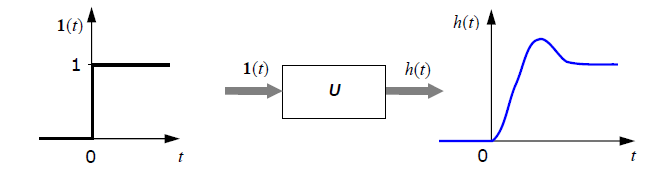
\includegraphics[width=0.7\textwidth]{24_perexod.png}
\caption{Реакция объекта на единичный скачок}
\end{figure}

При этом предполагается, что объект в начальный момент находится в состоянии покоя, то есть, имеет нулевые начальные условия. Это значит, что все его переменные состояния равны нулю и внутренняя энергия также нулевая. Если начальные условия ненулевые, то для построения сигнала выхода при любом входе нужно использовать дифференциальные уравнения объекта или модель в пространстве состояний. Это значит, что переходная характеристика дает меньше информации, чем исходные уравнения. Пусть модель объекта задана дифференциальным уравнением первого порядка:

\begin{eqnarray}
\centering
T\frac{dy(t)}{dt}+y(t)=k\cdot x(t)
\end{eqnarray} 
Где $k$---безразмерный коэффициент, а $T$---некоторая постоянная, которая имеет размерность времени. Найдем переходную характеристику этого звена. Решая уравнение при $x(t)=1 (t>0)$, получаем
\begin{eqnarray}
\centering
y(t)=k+C_{1}\cdot \exp\left(- \dfrac{t}{T}\right)
\end{eqnarray} 
Где постоянная $C_{1}$ должна определяться из начальных условий. Поскольку нас интересует переходная характеристика, начальные условия считаем нулевыми, то есть $y(0)=0$, что дает $C_{1}=-k$ и поэтому
\begin{eqnarray}
\centering
h(t)=y(t)=k\left[1-\exp\left(-\dfrac{t}{T}\right)\right]
\end{eqnarray} 
На рисунке показаны переходные характеристики при различных значениях параметра T, который называется постоянной времени звена:

\begin{figure}[H]
\centering
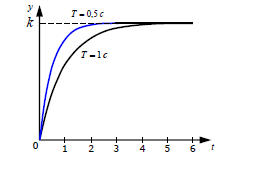
\includegraphics[width=0.6\textwidth]{24_graf.png}
\caption{Переходная характеристика}
\end{figure}

Видно, что при увеличении T выход y медленнее достигает значения, равного k , то есть постоянная времени характеризует инерционность звена. Чем больше постоянная времени, чем медленнее реагирует объект на управление и тем больше усилий нужно для того, чтобы перевести его в новое состояние. Заметим, что ступенчатый сигнал легко получить на практике, поэтому переходную характеристику можно снять экспериментально.

При единичном импульсном воздействии, входной сигнал равен нулю во всех точках, кроме t = 0 , где он уходит к бесконечность, причем его площадь (интеграл по всей оси времени) равен единице:

$$
1(t)=\left\{
		\begin{array}{r}
	 	0,t<0\\
		1,t\geq 0\\
		\end{array}
	\right.\;\;\;
\int\limits_{\infty}^{\infty}\delta(t)dt=1.	 		
$$ 

Реакция системы на единичный импульс (дельта-функцию) называется импульсной характеристикой и обозначается w(t):

\begin{figure}[H]
\centering
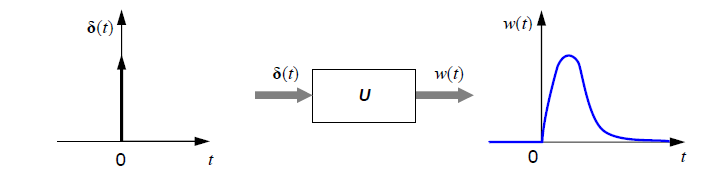
\includegraphics[width=0.6\textwidth]{24_impgraf.png}
\caption{Реакция объекта на импульсный скачок}
\end{figure}

Иногда определяют дельта-функцию как производную от единичного ступенчатого сигнала 1(t) . Действительно, эта производная равна нулю при всех значениях t , кроме нуля, где она обращается в бесконечность.

Пусть ширина прямоугольного импульса равна $\varepsilon$ , а высота –-- $1/\varepsilon$ . Такой импульс можно
представить в виде разности двух ступенчатых сигналов:

\begin{eqnarray}
x(t)=\dfrac{1}{\varepsilon}  \left[1(t)-1(t-\varepsilon)\right]
\end{eqnarray}

где $1(t\varepsilon)$ –-- это единичный ступенчатый сигнал, который приходит в момент $t=\varepsilon$ , то есть, смещен по времени на $\varepsilon$.

\begin{figure}[H]
\centering
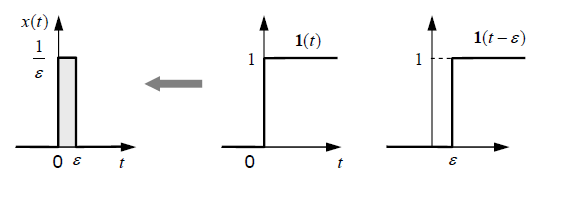
\includegraphics[width=0.6\textwidth]{24_imp.png}
\caption{Импульсное воздействие}
\end{figure}

Так как для линейных систем справедлив принцип суперпозиции, сигнал на выходе будет равен разности реакций системы на входы $1(t)$ и $1(t-\varepsilon)$ , умноженной на коэффициент $1/\varepsilon$ . Учитывая, что реакция на сигнал $1(t)$ –-- это переходная функция $h(t)$ , получаем:

\begin{eqnarray}
y(t)=\dfrac{1}{\varepsilon} \left[h(t)-h(t-\varepsilon)\right]
\end{eqnarray}

Переходя к пределу при $\varepsilon \rightarrow 0$, находим, что импульсная характеристика

\begin{eqnarray}
w(t)=\lim_{\varepsilon\rightarrow\infty}\frac{h(t)-h(t-\varepsilon)}{\varepsilon}=\dfrac{dh(t)}{dt}
\end{eqnarray}

как оказывается, равна производной от переходной функции. Наоборот, переходная функция – это интеграл от импульсной характеристики на интервале от 0 до t:

\begin{eqnarray}
h(t)=\int\limits_{0}^{t}w(\tau)d\tau
\end{eqnarray}

Дифференцируя переходную характеристику звена первого порядка, получаем соответствующую импульсную характеристику:
\begin{eqnarray}
w(t)=\dfrac{d}{dt}\left(k\left[1-\exp\left(-\dfrac{t}{T}\right)\right]\right)
\end{eqnarray}

Другое название импульсной характеристики – весовая функция. Это название связано с тем, что для произвольного входного сигнала x(t) выход системы y(t) при нулевых начальных условиях вычисляется как интеграл

\begin{eqnarray}
y(t)=\int\limits_{-\infty}^{t}x(\tau)w(t-\tau)d\tau=\int\limits_{0}^{\infty}(x(t-\tau)w(\tau)d\tau)
\end{eqnarray}

Здесь функция w(t) как бы «взвешивает» входной сигнал x(t) в подынтегральном выражении. Заметим, что импульсная характеристика дает неполную информацию об объекте, поскольку не учитывает ненулевые начальные условия. В отличие от ступенчатого сигнала, мгновенный импульс бесконечной величины невозможно получить на реальном устройстве, поэтому снять импульсную характеристику системы, строго говоря, экспериментально не удается.
 
% Вопрос 25 ---------------------------------------------------------------------------------------------------------------
\section{Типовые звенья САР и их частотные и временные характеристики.}

Типовые динамические звенья:
\begin{enumerate}
\item Усилительное звено. Усиливает в $ k $ раз.
	\begin{itemize}
	\item Передаточная функция:
		\begin{equation}
		w(s) = k.
		\end{equation}
	
	\item Переходная характеристика:
		\begin{equation}
		h(t) = k.
		\end{equation}

	\item Графики ($ \uparrow : k = 1, k = 5, k = 10 $):
	
	При увеличении коэффициента усиления увеличивается амплитуда, а фаза остаётся неизменной. Таким образом, усилительное звено увеличивает амплитуду входного сигнала. Амплитуда и фаза сигнала не зависят от частоты.
	
		\begin{figure}[H]
		\centering
		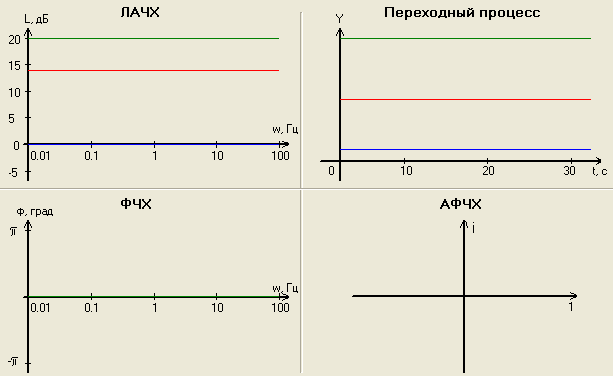
\includegraphics[width=0.7\linewidth]{25_usil.png}
		\caption{Временные и частотные характеристики звена}
		\end{figure}
	\end{itemize}


\item Апериодическое звено первого порядка. Наклон ЛАЧХ -20 дБ/дек.
	\begin{itemize}
	\item Передаточная функция:
		\begin{equation}
		w(s) = k \dfrac{1}{Ts + 1}.
		\end{equation}
	
	\item Переходная характеристика:
		\begin{equation}
		h(t) = k(1 - e^{-\frac{t}{T}}).
		\end{equation}

	\item Графики:
	
	Чем больше постоянная времени апериодического звена $ \tau $, тем быстрее убывает амплитуда выходного сигнала при одинаковых частотах. Чем больше $ \tau $, тем медленнее (плавнее) протекает переходный процесс. Фаза стремится к $ -\pi/2 $.
	
		\begin{figure}[H]
		\centering
		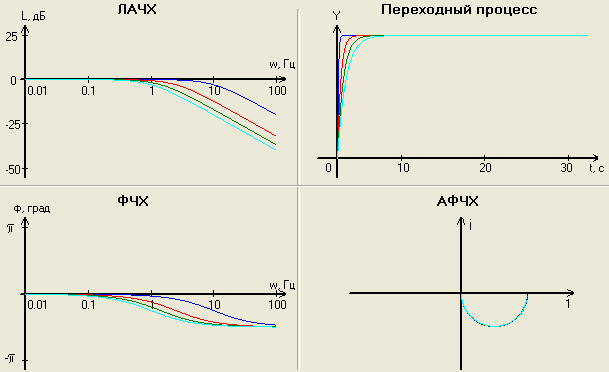
\includegraphics[width=0.75\linewidth]{25_ap1.png}
		\caption{Временные и частотные характеристики звена}
		\end{figure}
	\end{itemize}


\item Апериодическое звено второго порядка (колебательное). Наклон ЛАЧХ -40 дБ/дек.
	\begin{itemize}
	\item Передаточная функция:
		\begin{equation}
		w(s) = k \dfrac{1}{T^2s^2 + 2\xi T s + 1}\text{, где $ \xi $ --- ошибка, \textpm{}5\% }.
		\end{equation}
	
	\item Графики:
	
	Чем больше постоянная времени колебательного звена $ \tau $, тем быстрее убывает амплитуда выходного сигнала при одинаковых частотах. Чем больше $ \tau $, тем медленнее протекает переходный процесс. Фаза стремится к $ -\pi $.
	
		\begin{figure}[H]
		\centering
		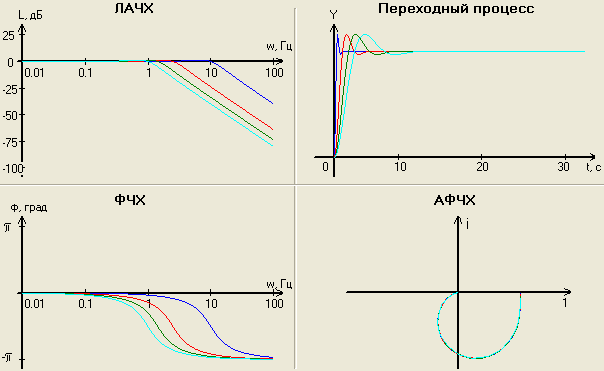
\includegraphics[width=0.75\linewidth]{25_ap2.png}
		\caption{Временные и частотные характеристики звена}
		\end{figure}
	\end{itemize}


\item Интегрирующее звено. Наклон ЛАЧХ -20 дБ/дек.
	\begin{itemize}
	\item Передаточная функция:
		\begin{equation}
		w(s) = \dfrac{1}{s}.
		\end{equation}
	
	\item Переходная характеристика:
		\begin{equation}
		h(t) = kt.
		\end{equation}
	
	\item Графики:
	
	Амплитуда выходного сигнала зависит от частоты и с её увеличением убывает. Фаза выходного сигнала не зависит от частоты и равна $ -\pi/2 $.
	
		\begin{figure}[H]
		\centering
		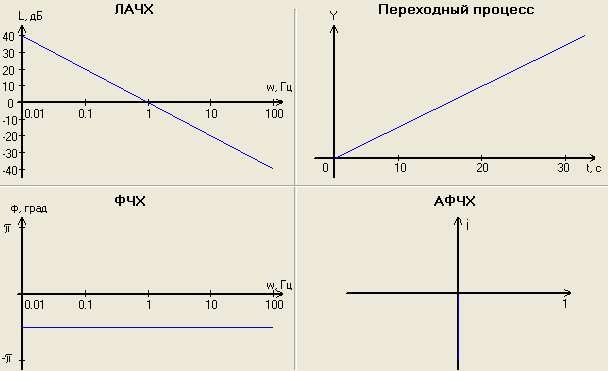
\includegraphics[width=0.75\linewidth]{25_integr.png}
		\caption{Временные и частотные характеристики звена}
		\end{figure}
	\end{itemize}



\item Дифференцирующее звено первого порядка. Наклон ЛАЧХ 20 дБ/дек.
	\begin{itemize}
	\item Передаточная функция:
		\begin{equation}
		w(s) = Ts + 1.
		\end{equation}
	
	\item Переходная характеристика:
		\begin{equation}
		h(t) = k [\tau \delta (t) + 1(t)].
		\end{equation}
	
	\item Графики:
	
	Чем больше постоянная времени звена $ \tau $, тем быстрее возрастает амплитуда выходного сигнала при одинаковых частотах. Чем больше $ \tau $, тем медленнее протекает переходный процесс. Фаза стремится к $ \pi/2 $.
	
		\begin{figure}[H]
		\centering
		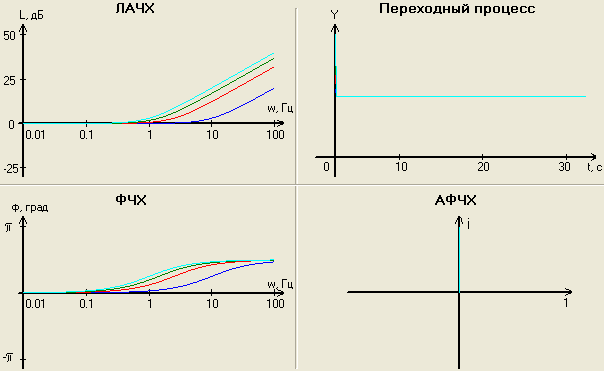
\includegraphics[width=0.75\linewidth]{25_dif1.png}
		\caption{Временные и частотные характеристики звена}
		\end{figure}
	\end{itemize}



\item Дифференцирующее звено второго порядка. Наклон ЛАЧХ 40 дБ/дек.
	\begin{itemize}
	\item Передаточная функция:
		\begin{equation}
		w(s) = T^2s^2 + 2\xi T s + 1.
		\end{equation}
	
	\item Графики:
	
	Чем больше постоянная времени звена $ \tau $, тем быстрее возрастает амплитуда выходного сигнала при одинаковых частотах. Чем больше $ \tau $, тем медленнее протекает переходный процесс. Фаза стремится к $ \pi $;
	
		\begin{figure}[H]
		\centering
		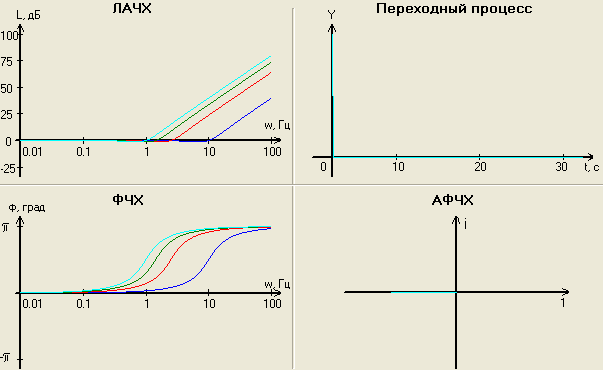
\includegraphics[width=0.75\linewidth]{25_dif2.png}
		\caption{Временные и частотные характеристики звена}
		\end{figure}
	\end{itemize}

\end{enumerate}



% Вопрос 26 ---------------------------------------------------------------------------------------------------------------
\section{Устойчивость линейных САР: определение, теоремы Ляпунова, алгебраический критерий устойчивости Гурвица.}

Система считается \textit{устойчивой}, если отклонение выходной величины, возникшей в результате внешнего возмущения, по истечении некоторого времени становится меньше заданного.

\begin{equation}
\lim\limits_{t\rightarrow\infty} |X_\text{вых}(t)| \leq \varepsilon
\end{equation}

Таким образом, если САР выведена из состояния равновесия, а затем предоставлена самой себе, то она должна возвратится в состояние равновесия.

Ляпунов доказал 2 теоремы:
\begin{enumerate}
\item Если вещественные части всех корней характеристического уравнения 1-го приближения отрицательные, то собственное движение асимптотически устойчиво независимо от членов разложения выше 1-го порядка малости
\item Если среди корней характеристического уравнения 1-го приближения найдется по меньшей мере один с положительной вещественной частью, то собственное движение неустойчиво независимо от членов разложения выше 1-го порядка малости.
\end{enumerate}

Критические случаи имеют место, когда среди корней имеются корни с нулевой вещественной частью. Тогда вопрос об устойчивости необходимо решать исследованием полного нелинейного дифференциального уравнения.

\subsection*{Алгебраический критерий устойчивости Гурвица.}

Устойчивость замкнутой динамической системы, имеющей характеристическое уравнение $ D_3(s) = a_n s^n + a_{n-1} s^{n-1} + \ldots + a_1 s + a_0 $ определяется выполнением следующих условий:
\begin{enumerate}
\item коэффициенты характеристических уравнений положительны (необходимое условие);
\item диагональные миноры больше нуля (достаточное условие).
\end{enumerate}

\begin{figure}[H]
\centering
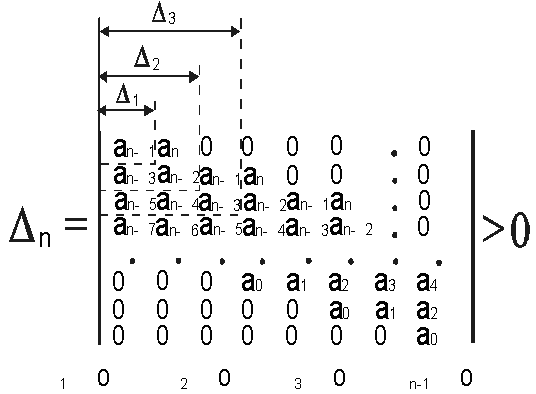
\includegraphics[width=0.5\linewidth]{26_matrix.png}
\caption{Матрица Гурвица}
\end{figure}

Определитель $ \Delta_n $ составляется следующим образом: главная диагональ состоит из коэффициентов характеристического уравнения записанных начиная со второго ($ a_{n-1} $). Строки заполняются следующим образом: в левую сторону от основной диагонали записываются коэффициенты в порядке убывания индексов, в правую --- в порядке возрастания. Остальные ячейки заполняются нулями.

\textbf{Например}, характеристическое уравнение имеет вид:
$$ 0,05 \cdot s^3 + 0,15 \cdot s^2 + 0,7 \cdot s + 1 = 0. $$

Все коэффициенты характеристического уравнения положительны, следовательно необходимое условие устойчивости системы выполняется.

Матрица Гурвица запишется как:
$$
\begin{pmatrix}
a_2 & a_3 & 0   \\
a_0 & a_1 & a_2 \\
0   & 0   & a_0 \\
\end{pmatrix}
\quad = \quad
\begin{pmatrix}
0,15	& 0,05	& 0		\\
1		& 0,7	& 0,15	\\
0		& 0		& 1		\\
\end{pmatrix}.
$$

\par $ \Delta_1 = a_2 =  0,05 > 0.$
\par $ \Delta_2 = a_2 a_1 - a_3 a_0 =  0,15 \cdot 0,7 - 0,05 = 0,055 > 0.$
\par $ \Delta_3 = a_2 a_1 a_0 - a_0 a_3 a_0 = 0,15 \cdot 0,7 - 0,05 = 0,055 > 0.$

Достаточное условие так же выполняется (все диагональные миноры больше нуля), следовательно САУ с таким характеристическим уравнением является устойчивой.

% Вопрос 27 ---------------------------------------------------------------------------------------------------------------
\section{Частотные критерии устойчивости линейных САР.}

\subsection*{Амплитудно-фазовый критерий устойчивости (Найквиста-Михайлова).}

Критерий получил наибольшее распространение в инженерной практике так как позволяет определить устойчивость замкнутой системы по её поведению в разомкнутом состоянии.

Пусть $ L(s) $ – передаточная функция разомкнутой системы, а $ L(j\omega) $ – ее частотная характеристика.
%Характеристическое уравнение замкнутой системы может быть представлено в следующем виде:
%\begin{equation}
%W(s) + 1 = \dfrac{M(s) + D(s)}{D(s)} = \dfrac{D_3(s)}{D(s)} = 0.
%\end{equation} % Што за бред?

Для каждой частоты $ \omega $ значение $L(j\omega)$ – это комплексное число, которое можно изобразить точкой на комплексной плоскости. При изменении частоты от 0 до $ \infty $ из этих точек складывается годограф Найквиста – некоторая кривая, которая начинается в точке (K; 0) на вещественной оси и заканчивается в начале координат (если $ L(s) $ – строго правильная функция, то есть степень ее числителя меньше степени знаменателя). Можно доказать, что система устойчива тогда и только тогда, когда годограф $L(j\omega)$ не охватывает точку (-1; 0).

%Результирующий вектор:
%\begin{equation}
%\overline{W(j\omega) + 1} = \overline{W(j\omega)} + \overline{1}.
%\end{equation}

\begin{figure}[H]
\centering
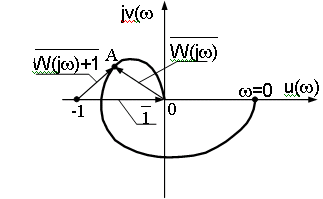
\includegraphics[width=0.3\linewidth]{27_mih_nike.png}
\caption{АФХ разомкнутой системы}
\end{figure}

Выражение «система находится на границе устойчивости» означает, что частотная характеристика проходит через точку (-1; 0). 

В этом случае для некоторой частоты $ \omega $ мы имеем $A(\omega) =1$ и $\varphi(\omega) = -180^\circ$ . Это говорит о том, что после прохождения контура величина сигнала меняет знак, сохраняя абсолютную величину (энергию), то есть устанавливаются незатухающие колебания. Частота, на которой это происходит, называется частотой среза. Для устойчивой системы значение фазы на частоте среза должно быть больше, чем $ -180^\circ $.

\subsection*{Критерий  D-разбиения}

Метод позволяет построением одной кривой выявить сразу все значения интересующего параметра, при котором САР остается устойчивой.

Параметры САР могут быть разбиты на 3 группы:
\begin{enumerate}
\item заданные, которые обеспечиваются конструкцией системы;
\item конструктивные, которые могут быть изменены в определенных пределах;
\item настроечные.
\end{enumerate}

\subsection*{D-разбиение по одному параметру}

Пусть необходимо выявить влияние на устойчивость САУ, например, коэффициента усиления $ K $. Приведем характеристическое уравнение к виду $ D(p) = S(p) + KN(p) $, выделив члены, не зависящие от $ K $ в полином $ S(p) $, а в остальных членах, линейно зависящих от $ K $, вынесем его за скобки. Граница D-разбиения задается уравнением:

%Характеристическое уравнение $ a_n s^n + a_{n-1} s^{n-1} + \ldots + a_1 s + a_0 = 0 $ всегда может быть представлено в следующем виде $ \mu S(s) + V(s) = 0 $, где $ \mu $ --- искомый параметр:
%\begin{equation}
%\mu = \dfrac{N(s)}{S(s)} = -\dfrac{N(j\omega)}{S(j\omega)} = A(\omega) = -jB(\omega).
%\end{equation}

\begin{equation}
D(j\omega)=S(j\omega)+KN(j\omega)=0, \Rightarrow K= -\dfrac{S(j\omega)}{N(j\omega)} = X(\omega) + jY(\omega)
\end{equation}

\begin{figure}[H]
\centering
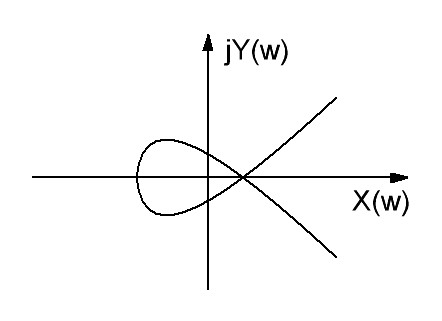
\includegraphics[width=0.4\linewidth]{27_d.jpg}
\caption{Пример кривой D-разбиения}
\end{figure}

Задаваясь $ \omega $ от $ -\infty $ до $ +\infty $, вычисляют $X(\omega)$ и $Y(\omega)$ и строят на комплексной плоскости кривую $ D $-разбиения. При движении от $ -\infty $ до $ +\infty $ область корней с отрицательными вещественными частями остается слева, левую сторону кривой заштриховывают. Полученная кривая представляет собой границу устойчивости (ее можно рассматривать также как отображение мнимой оси плоскости корней). Эта кривая симметрична относительно вещественной оси, поэтому достаточно построить ее часть, соответствующую положительным значениям частоты, а вторую часть получить отображением относительно вещественной оси.

Кривая D разбивает плоскость параметра на несколько областей с различным условием устойчивости, для определения которого необходимо выбрать по одному значению D в каждой из них и проверить устойчивость с помощью какого-либо критерия. Если система устойчива при выбранном D, то она будет устойчива и при других значениях из этой области.

Есть одна особенность. Так как $ K $ - вещественное число, то $ Y(\omega) = 0 $, поэтому нас интересует не вся область устойчивости, а лишь отрезок вещественной оси в этой области, то есть $ K = X(\omega) $.
%Поскольку $ \mu $ --- действительные параметры САР, рассматриваются только точки действительной оси $ A(\omega) $, расположенные по левую сторону $ D $-кривой. Выбранные значения $ \mu $ проверяем по какому-либо критерию устойчивости.


% Вопрос 28 ---------------------------------------------------------------------------------------------------------------
\section{Анализ качества линейных САР.}

Задача анализа качества процесса регулирования заключается в нахождении ряда показателей, характеризующих переходную характеристику системы и названных первичными показателями качества.

Методы анализа качества:
\begin{itemize}
\item Частотный. Основан на рассмотренном преобразовании Лапласа $ X_\text{вых}(s) $ при $ s = j\omega $, а также на связи между частотными характеристиками замкнутых (разомкнутых) систем и переходными характеристиками.
\item Корневого годографа. Метод не требует определения корней характеристического уравнения, является графоаналитическим.
\item Логарифмического корневого годографа.
\item Интегральных оценок.
\item Косвенный. Основан на вычислении определенных интегралов по времени. Эффективен при использовании ЭВМ.
\end{itemize}

\subsection*{Частотный метод}

\begin{wrapfigure}{o}{0.45\textwidth}
\centering
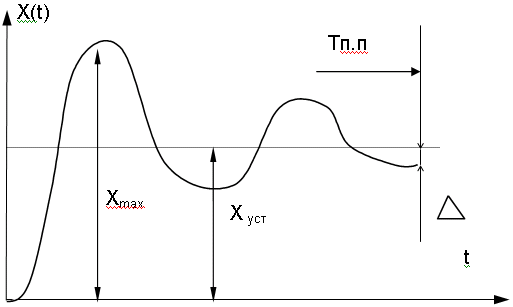
\includegraphics[width=\linewidth]{28_proc.png}
\caption{Переходный процесс}
\end{wrapfigure}

На рисунке представлены показатели характеризующие устойчивость системы.

\begin{enumerate}
\item Установившееся значение $ X_\text{уст} = X(\infty) $ определяет статическую точность системы.\\ $ E_\text{уст} = X_\text{вх} - X_\text{уст} $
\item Время перехода процесса $ T_\text{п.п.} $ определяется как наименьшее значение интервала времени, в течение которого $ [X(t)- X_\text{уст}] \leq \Delta $, где $ \Delta $ заданная постоянная малая величина (обычно$  \Delta = 0,05 X_\text{уст} $).
\item Положительное перерегулирование\\ $ \sigma = \dfrac{X_\text{max} - X_\text{уст}}{X_\text{уст}} \cdot 100\% $.
\item Число колебаний $ N $ величины $ X(t) $ в течение времени $ T_\text{п.п.} $.
\end{enumerate}

\subsection*{Определение переходных процессов}

\begin{enumerate}
\item Аналитический метод.

Если $ P_\text{З}(\omega) $ и $ Q_\text{З}(\omega) $ заданы аналитически, то удобно $ h(t) $ определять численными методами с использованием ЭВМ. Удобно использовать метод Филона интегрирования осциллирующих функций $ f(\omega) = \sin\omega t $.


\item Графоаналитический метод (метод трапецеидальных частотных характеристик).

Для построения $ P_\text{З}(\omega) $ и $ Q_\text{З}(\omega) $ применяются номограммы. Кривая $ P(\omega) $ может быть представлена в виде совокупности из некоторого числа трапецеидальных частотных характеристик:
\begin{equation}
P(\omega) \approx \sum_{i=1}^{n} r_i(\omega).
\end{equation}

Этой сумме соответствует $ h(t) $, являющееся линейной комбинацией функции $ h_i(t) $:
\begin{equation}
h(t) = \sum_{i=1}^{n} h_i(t).
\end{equation}

$ h_i(t) $ определяется по типовой вещественной частотной характеристике.
\end{enumerate}


% Вопрос 29 ---------------------------------------------------------------------------------------------------------------
\section{Синтез корректирующих устройств линейных САР.}

В автоматике применяют следующие способы коррекции динамических характеристик:
\begin{enumerate}
\item Последовательная коррекция (последовательно в прямой цепи).
\item Параллельная коррекция (параллельно прямой цепи).
\item С помощью корректирующей обратной связи (КОС).
\item Комбинированная.
\end{enumerate}

Корректирующие обратные связи уменьшают зависимость динамических свойств от изменения параметров элементов, уменьшают влияние помех но имеют высокую стоимость и громоздкость (тахогенераторы, вращающие трансформаторы).

Проектирование САР сводится к следующим этапам:
\begin{enumerate}
\item проектирование не скорректированной САР из условий физической осуществимости;
\item проектирование идеальной модели системы (желаемая характеристика);
\item компенсирование различий этих систем с помощью корректирующих цепей.
\end{enumerate}

Синтез корректирующей цепи заключается в выборе ее вида, определении передаточной функции, расчете параметров цепи.

\subsection*{Построение желаемой ЛАХ}

Порядок определения желаемой ЛАХ:
\begin{enumerate}
\item Низкочастотная асимптота проходит под наклоном $ -20\nu $ дБ/дек, где $ \nu $ --- порядок астатизма, а при частоте имеет ординату $ 20\lg k $ (дБ).
\item По заданному значению $ \sigma_\text{max} = f(P_\text{max}) $ определяет значение $ P_\text{max} $.
\par Значение $ [P_\text{min}) \approx P_\text{max} - 1 $.


\item Определяют частоту среза $ \omega_\text{ср. Tmax.} < \omega_\text{ср} < \omega_\text{ср. опт.} $, где $ \omega_\text{ср. опт.} = \sqrt{\dfrac{\omega_\text{max}}{g_0}} $.
\par $ \omega_\text{ср. опт.} $ --- заданное максимальное ускорение объекта регулирования.
\par $ \omega_\text{ср. Tmax.} $ находят по кривой $ T_\text{max} = f_1(T_\text{max}) $ при значении $ P_\text{max} $ из п.2.

\item Через точку $ \omega_\text{ср.} $  проводят среднечастотную асимптоту с наклоном -20 дБ/дек.
\item Производят сопряжение среднечастотной асимптоты с низкочастотной:
	\begin{enumerate}
	\item если в ТЗ задана точность и порядок астатизма, то $ \omega_1 \approx 0,15\omega_\text{n} $.
	\item если требования точности не определены, то сопряжение начинают с $ L_2\omega $ = +16 дБ.
	\end{enumerate}

\item Проверяют запасы устойчивости по модулю и фазе.
\item Строят высокочастотную асимптоту так, чтобы она мало отличалась от нескорректированной САР, желательно $ L_3 \approx -L_2 $.

\begin{figure}[H]
\centering
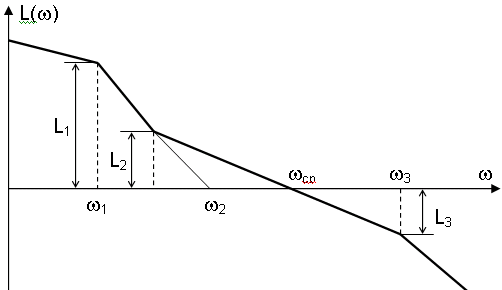
\includegraphics[width=0.5\linewidth]{29_lachh.png}
\caption{Желаемая ЛАЧХ}
\end{figure}

\end{enumerate}

\textit{Синтез КОС} может осуществляться отрицательной жесткой ОС или гибкой ОС(связью по производным).

Жесткие ООС уменьшают статический коэффициент усиления охватываемых участков, увеличивают устойчивость и ошибки в установившемся состоянии.

Охват инерционных звеньев жёсткой обратной связи (ЖОС) приводит к снижению инерционности.

Гибкие ОС (связи по производным) не оказывает влияние на статический коэффициент усиления охватываемых участков и эффективно воздействуют на форму переходных процессов и устойчивость.

Для определения $ Z(s) $ применяются следующие способы: 
\begin{enumerate}
\item эквивалентной последовательной коррекции.
\par Из условия эквивалентности
$ W_\text{пос} W_\text{охв} W_\text{неохв}  = \dfrac{W_\text{неохв} W_\text{охв}}{1 + W_\text{охв} Z} $, поэтому 
$ Z = \dfrac{1 - W_\text{пос}}{W_\text{охв} W_\text{пос}} $.
\par При таком подходе может получится физически не реализуемая передаточная функция.
\item В заданном интервале частот $ [\omega_1, \omega_2] $ обеспечивают $ ( W_\text{охв} Z ) >> 1 $, тогда  и для выполнения условия  $ (W_\text{охв} Z)  >> 1 $ вводят последовательное усилительное звено $ W(j\omega) = \dfrac{W_\text{неохв}(j\omega)}{Z(j\omega)} $.
\end{enumerate}


% Вопрос 30 ---------------------------------------------------------------------------------------------------------------
\section{Анализ нелинейных САР.}

Для анализа нелинейных систем применяются методы: фазовых траекторий, припасовывания, гармонической линеаризации, фазовой границы устойчивости и др.

\subsection*{Метод фазовых траекторий}

Фазовой плоскостью называется плоскость на которой по двум координатам X и Y откладываются какие-либо две переменные, характеризующие динамику САР, например отклонение регулируемой величины $ X $ и скорость $ X = Y = dx/dt $.

Уравнение второго порядка удобно свести к системе двух уравнений первого порядка:
\begin{equation}
\dfrac{dx}{dt} = f_1(x, y) \quad \dfrac{dy}{dt} = f_2(x, y).
\end{equation}

Для изображения на фазовой плоскости исключается время t, для чего второе делят на первое:
\begin{equation}
\dfrac{dx}{dy} = \dfrac{f_1(x, y)}{f_2(x, y)}.
\end{equation}

Получаем нелинейное дифференциальное уравнение, решение которого $ Y = F(x) $ называется \textit{фазовой траекторией}.

Для САР, линейная часть которой имеет порядок > 2, применяются \textit{многолистные фазовые плоскости}.

\subsection*{Изображения процессов регулирования на фазовой плоскости.}

\begin{enumerate}
\item Периодический незатухающий колебательный процесс.

\begin{eqnarray}
x(t) = a \sin(\omega t)			&\quad& \sin^2(\omega t) = x^2 / a^2 ;\\
y(t) = a\omega \cos (\omega t)	&\quad& \cos^2(\omega t) = y^2 / a^2 \omega^2;
\end{eqnarray}

\begin{equation}
\dfrac{x^2}{a^2} + \dfrac{y^2}{a^2 \omega^2} = 1.
\end{equation}

\begin{figure}[H]
\centering
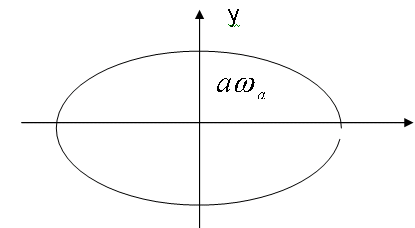
\includegraphics[width=0.4\linewidth]{30_per_nez.png}
\caption{Периодический колебательный процесс}
\end{figure}


\item Затухающий колебательный процесс.

\begin{equation}
x(t) = ae^{-nt} \cos \omega t;
\end{equation}
\begin{equation}
y(t) = ae^{-nt} \sqrt{\omega^2 + n^2} \sin[\omega t + \varphi(t) ].
\end{equation}

\begin{figure}[H]
\centering
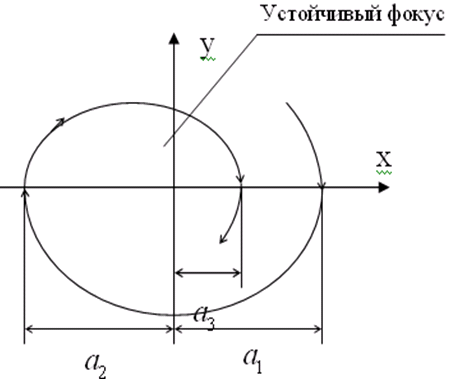
\includegraphics[width=0.4\linewidth]{30_coleb_zat.png}
\caption{Колебания с убывающей амплитудой}
\end{figure}


\item Расходящийся колебательный процесс.

\begin{equation}
x(t) = ae^{nt} \cos \omega t;
\end{equation}
\begin{equation}
y(t) = ae^{nt} \sqrt{\omega^2 + n^2} \sin[\omega t + \varphi(t) ].
\end{equation}

\begin{figure}[H]
\centering
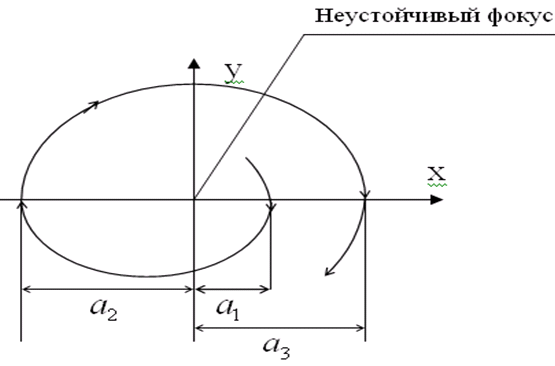
\includegraphics[width=0.4\linewidth]{30_coleb_rash.png}
\caption{Колебания с возрастающей амплитудой}
\end{figure}


\item Затухающие апериодические процессы.

\begin{figure}[H]
\centering
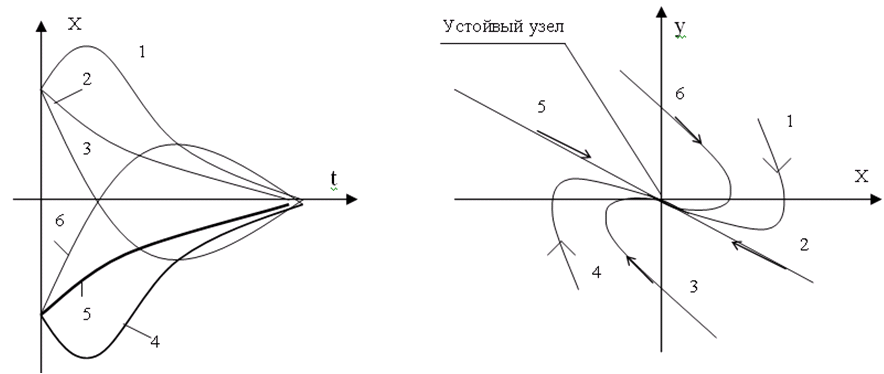
\includegraphics[width=0.8\linewidth]{30_aperiod_zat.png}
\caption{Переходный процесс и фазовая траектория затухающих апериодических процессов}
\end{figure}


\item Расходящиеся апериодические процессы.

\begin{figure}[H]
\centering
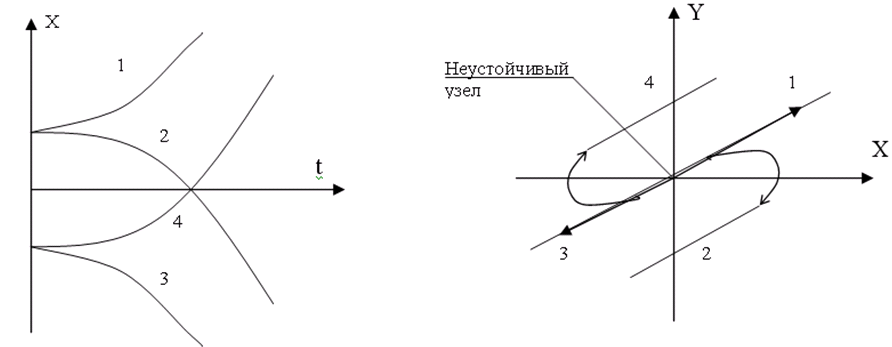
\includegraphics[width=0.8\linewidth]{30_aperiod_rash.png}
\caption{Переходный процесс и фазовая траектория расходящихся апериодических процессов}
\end{figure}

\end{enumerate}

\end{document}